\documentclass{beamer}

\setlength{\parskip}{\baselineskip}
\setlength{\parindent}{0pt}
\usepackage{default}
\usepackage{tabularx}
\usepackage{url}
\usepackage{graphicx}
\usepackage{tikz}
\usepackage{pgfplots}
\usepackage{color}

\pgfplotscreateplotcyclelist{my_style}{%
teal,every mark/.append style={fill=teal!80!black},mark=*\\%
orange,every mark/.append style={fill=orange!80!black},mark=square*\\%
cyan!60!black,every mark/.append style={fill=cyan!80!black},mark=diamond*\\%
red!70!white,densely dashed,mark=star\\%
lime!80!black,densely dashed,every mark/.append style={solid,fill=lime},mark=diamond*\\%
red,densely dashed,every mark/.append style={solid,fill=red!80!black},mark=otimes*\\%
% yellow!60!black,densely dashed,
% every mark/.append style={solid,fill=yellow!80!black},mark=square*\\%
% black,every mark/.append style={solid,fill=gray},mark=otimes*\\%
% blue,densely dashed,mark=star,every mark/.append style=solid\\%
% red,densely dashed,every mark/.append style={solid,fill=red!80!black},mark=diamond*\\%
}

\title{\huge{Why PGFPlots is better than Matlab's figures?}}
\author{Manuel Baumann}
\titlegraphic{
   \vspace{-1cm}
   
\includegraphics[scale=0.08]{images/TU_Delft_logo1.png}\hspace{4cm}\includegraphics[scale=0.15]{../../images/logo}}
\date{\footnotesize{September 24, 2015}}
\begin{document}

\frame{\titlepage}
\begin{frame}
\frametitle{What is PGFPlots ?}
A plot in a high-end \LaTeX \ document should:
\begin{itemize}
 \item be font-consistent,
 \item be high-quality,
 \item be based on (scientific) data,
 \item be scalable.
\end{itemize}
\pause
Hence, \texttt{PGFPlots} is what you need...
\end{frame}

\begin{frame}
\frametitle{Example: The young Manuel...}
\begin{figure}
 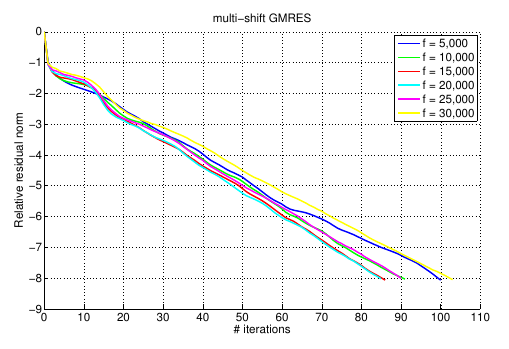
\includegraphics[width=0.8\textwidth]{images/matlab.png}
\end{figure}
\end{frame}

\begin{frame}
\frametitle{Example: How it looks in SISC}
\begin{figure}
 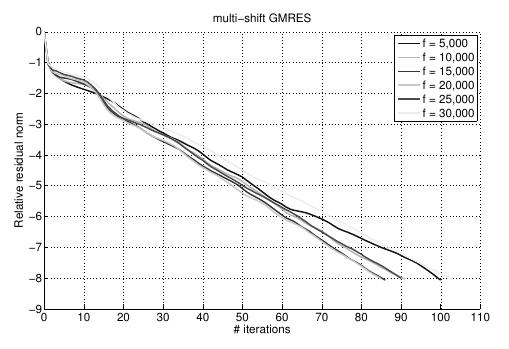
\includegraphics[width=0.8\textwidth]{images/matlab_bw.png}
\end{figure}
\end{frame}

\begin{frame}
\frametitle{Example: How it REALLY looks in SISC}
\begin{figure}
 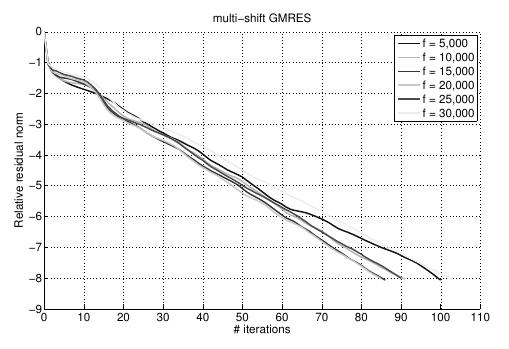
\includegraphics[width=0.4\textwidth]{images/matlab_bw.png} \hspace{0.6cm} 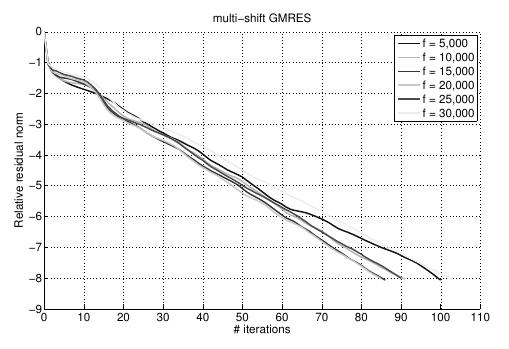
\includegraphics[width=0.4\textwidth]{images/matlab_bw.png} 
\end{figure}
\end{frame}

\begin{frame}
\frametitle{Example: What PGFPlots can do...}
\centering
\begin{tikzpicture} 
\begin{semilogyaxis}[width = 0.8\textwidth, 
%                      height = 10cm,
                     title={Convergence of multi-shift GMRES},
                     xlabel={\# iterations},
                     xmin = 1,
                     xmax = 103,
%                      xtick={0,...,9},
                     ylabel={Relative residual norm},
                     ymax = 1,
                     ymin = 1e-8,
                     grid=major,
                     mark repeat={5},
                     cycle list name=my_style] 
                     
\addplot table [x = {iters}, y = {f1}] {resvec.dat};
\addplot table [x = {iters}, y = {f2}] {resvec.dat};
\addplot table [x = {iters}, y = {f3}] {resvec.dat};
\addplot table [x = {iters}, y = {f4}] {resvec.dat};
\addplot table [x = {iters}, y = {f5}] {resvec.dat};
\addplot table [x = {iters}, y = {f6}] {resvec.dat};

% \addplot[color=black,dashed] coordinates { (0,0.1) (170,0.1)}; % inner trashhold
\legend{$f_1=\phantom{0}5$ Hz,$f_2=\phantom{0}6$ Hz,$f_3=\phantom{0}7$ Hz,$f_4=\phantom{0}8$ Hz,$f_5=\phantom{0}9$ Hz,$f_6=10$ Hz} 

\end{semilogyaxis} 
\end{tikzpicture}
\end{frame}

\begin{frame}[fragile]
\frametitle{Example: What PGFPlots can do...}
\begin{verbatim}
 \begin{semilogyaxis}[width  = 12cm, 
                      height = 10cm,
                      title  = {multi-shift GMRES},
                      xlabel = {\# iterations},
                      ylabel = {Relative residual norm},
                      xmin   = 1,
                      xmax   = 103,
                      ymax   = 1,
                      ymin   = 1e-8,
                      grid   = major,
                      mark repeat = {5},
                      cycle list name = my_style ] 
                     
\addplot table [x = {iters}, y = {f1}] {resvec.dat};
\addplot table [x = {iters}, y = {f2}] {resvec.dat};
\legend{$f_1=5$ Hz,$f_2=6$ Hz} 
\end{verbatim}
\end{frame}

\begin{frame}{More examples (C. Feuers\"anger)}
    \begin{itemize}
        \item \url{http://pgfplots.sourceforge.net}
     \end{itemize}
 \includegraphics[width=50pt]{pgfplots_talk_FTUG_2012/title/example_106.pdf} 
 \includegraphics[width=50pt]{pgfplots_talk_FTUG_2012/title/example_114.pdf} 
 \includegraphics[width=50pt]{pgfplots_talk_FTUG_2012/title/example_150.pdf} 
 \includegraphics[width=50pt]{pgfplots_talk_FTUG_2012/title/example_151.pdf} 
 \includegraphics[width=50pt]{pgfplots_talk_FTUG_2012/title/example_154.pdf} 
 \includegraphics[width=50pt]{pgfplots_talk_FTUG_2012/title/example_185.pdf}

 \includegraphics[width=50pt]{pgfplots_talk_FTUG_2012/title/example_99.pdf}
 \includegraphics[width=50pt]{pgfplots_talk_FTUG_2012/title/example_193.pdf} 
 \includegraphics[width=50pt]{pgfplots_talk_FTUG_2012/title/example_25.pdf} 
 \includegraphics[width=50pt]{pgfplots_talk_FTUG_2012/title/example_272.pdf} 
 \includegraphics[width=50pt]{pgfplots_talk_FTUG_2012/title/example_323.pdf} 
 \includegraphics[width=50pt]{pgfplots_talk_FTUG_2012/title/example_42.pdf} 

 \includegraphics[width=50pt]{pgfplots_talk_FTUG_2012/title/example_433.pdf} 
 \includegraphics[width=50pt]{pgfplots_talk_FTUG_2012/title/example_452.pdf} 
 \includegraphics[width=50pt]{pgfplots_talk_FTUG_2012/title/example_4.pdf} 
 \includegraphics[width=50pt]{pgfplots_talk_FTUG_2012/title/example_76.pdf} 
 \includegraphics[width=50pt]{pgfplots_talk_FTUG_2012/title/example_8.pdf} 
 \includegraphics[width=50pt]{pgfplots_talk_FTUG_2012/title/example_92.pdf} 
\end{frame}

\begin{frame}
\frametitle{Further reading}
Many information are available online:
\begin{itemize}
 \item \url{http://pgfplots.sourceforge.net/}
 \item \url{http://pgfplots.sourceforge.net/gallery.html}
 \item \small{\url{http://wissrech.ins.uni-bonn.de/people/feuersaenger/}}
\end{itemize}
These slides, and much more, will be published at:
\begin{itemize}
 \item \url{http://projectbanana.github.io/}
\end{itemize}
 \begin{figure}
\centering
 \includegraphics[height=0.3\textheight]{../../images/logo}
\end{figure}
\end{frame}

\begin{frame}
\frametitle{We need to talk about...}
\vspace{0.5cm}
Short report of 2014-15:
\begin{itemize}
 \item I count \# 63 members
 \item $500 \$$ are spent \texttt{:P}
 \item We did: \href{http://sinews.siam.org/DetailsPage/tabid/607/ArticleID/504/European-Students-Gather-at-TU-Delft-for-Krylov-Day.aspx}{SSC Krylov Day}, TATA Steel visit, BBQ, movie night, baNaNa talks, Mathias' seminar, ...
\end{itemize}

Ideas for the new academic year:
\begin{itemize}
 \item new webmaster ... who{\color{red}?}
 \item more baNaNa talks ... who{\color{red}?}
 \item $SIAM \ CFD^2ay \ 2016$ (Thea {\color{red}?}), \\ Modeling Day (Behrouz {\color{red}?}), ...
 \item chess competition (Reinaldo {\color{red}?})
\end{itemize}
 \vspace{-3cm}
 \begin{figure}
 \hfill
 
\includegraphics[height=0.3\textheight]{images/SIAMSC_Delft}
\end{figure}
\end{frame}

\end{document}
